\documentclass[12pt]{article}
\usepackage[margin=2.5cm]{geometry}
\usepackage{enumerate}
\usepackage{amsfonts}
\usepackage{amsmath}
\usepackage{fancyhdr}
\usepackage{amsmath}
\usepackage{amssymb}
\usepackage{amsthm}
\usepackage{mdframed}
\usepackage{graphicx}
\usepackage{subcaption}
\usepackage{listings}
\usepackage{xcolor}
\usepackage{booktabs}
\usepackage[utf]{kotex}

\definecolor{codegreen}{rgb}{0,0.6,0}
\definecolor{codegray}{rgb}{0.5,0.5,0.5}
\definecolor{codepurple}{rgb}{0.58,0,0.82}
\definecolor{backcolour}{rgb}{0.95,0.95,0.92}

\lstdefinestyle{mystyle}{
    backgroundcolor=\color{backcolour},
    commentstyle=\color{codegreen},
    keywordstyle=\color{magenta},
    numberstyle=\tiny\color{codegray},
    stringstyle=\color{codepurple},
    basicstyle=\ttfamily\footnotesize,
    breakatwhitespace=false,
    breaklines=true,
    captionpos=b,
    keepspaces=true,
    numbers=left,
    numbersep=5pt,
    showspaces=false,
    showstringspaces=false,
    showtabs=false,
    tabsize=1
}

\lstset{style=mystyle}

\begin{document}
\title{CSC148 Worksheet 11 Solution}
\author{Hyungmo Gu}
\maketitle

\section*{Question 1}
\begin{enumerate}[a.]
    \item Here, the constant time means the running time of accessing and
    assigning element by index doesn't depend on the length of the list.

    \item

    \begin{align*}
        n -i
    \end{align*}

    many elements need to be shifted to right.

    \bigskip

    \underline{\textbf{Notes:}}

    \bigskip

    \begin{itemize}
        \item

        The following example tells us

        \begin{center}
        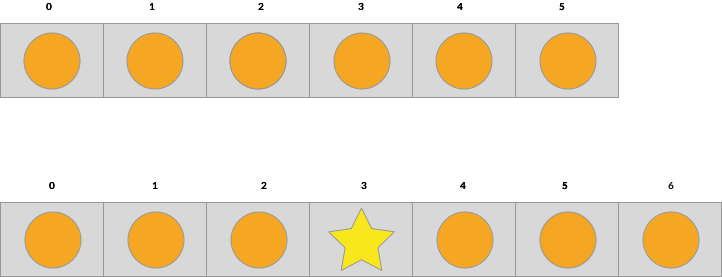
\includegraphics[width=0.8 \linewidth]{images/worksheet_11_q1b_notes.png}
        \end{center}

        to position an element at index $i = 3$ of the list, $n - i = 6 - 3 = 3$
        elements must be moved over.

        \bigskip

        Using this fact, we can generalize that to position an element at index $i$
        of the list, $n - i$ many elements must be shifted.

        \item Learned that when items shifts, it shifts into the expansion room.

        \begin{center}
        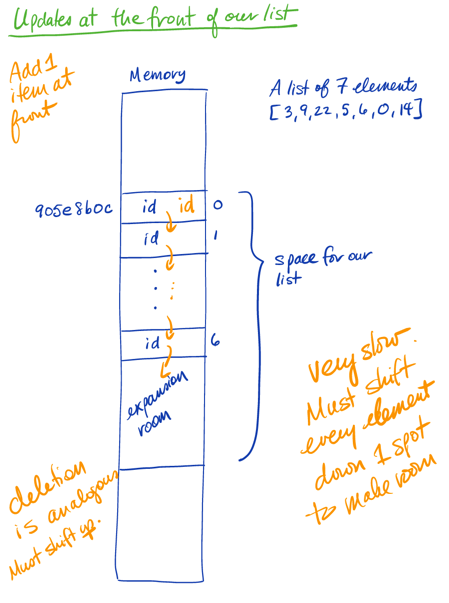
\includegraphics[width=0.8 \linewidth]{images/worksheet_11_q1b_notes2.png}
        \end{center}
    \end{itemize}

    \item Because we know the list size stays as is when an element is removed, we can
    conclude 0 many list elements must be moved.

    \bigskip

    \begin{mdframed}
        \underline{\textbf{Correct Solution:}}

        \color{red}
        The following example tells us

        \begin{center}
        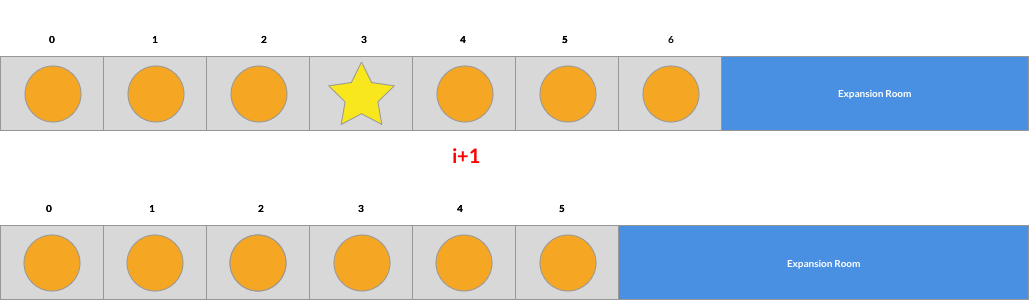
\includegraphics[width=\linewidth]{images/worksheet_11_q1c_correction.png}
        \end{center}

        when an element at index $i = 3$ is removed from the list $n - (i+1) =
        7 - (3 - 1) = 3$ many elements must be moved.

        \bigskip

        Using this fact, we can generalize that when an element is removed,
        $n - (i+1) = n - i - 1$ many elements must be shifted to left.

        \color{black}

    \end{mdframed}

    \item

    \begin{enumerate}[i.]
        \item

        A solution is \textit{LIST.remove(...)}.

        \bigskip

        The answer to question 1.d tells us when an element is removed, $n-i$
        must be shifted to left.

        \bigskip

        Using this fact, we can write a list of smaller size needs to shift elements less.

        \bigskip

        Then, it follows from this fact that $n = 100$ works faster than $n = 1,000,000$.

        \item

        A solution is \textit{LIST.append(...)}

        \bigskip

        The definition of append tells us that upon call, an element is added to
        the end of a list, it takes a constant time to add an element
        as long as the expansion room is not filled.

        \bigskip

        It follows from this fact that $n = 100$ and $n = 1,000,000$ takes roughly
        the same amount of time.
    \end{enumerate}

\end{enumerate}

\section*{Question 2 }

\end{document}